\section{Introduction}

\indent In this technical report we present a series of design directions for the development of open-source, affordable robot hands, that are also:

\begin{itemize}
	\item{modular}
	\item{light-weight}
	\item{intrinsically-compliant}
	\item{underactuated}
\end{itemize}
 
The following sections describe how to construct a series of robot hands with the aforementioned features. For their development we use off-the-shelf materials and equipment that can be easily found in hardware stores. The proposed robot hands, efficiently grasp a series of everyday life objects and are considered to be general purpose, as they can be used for various applications. 

\begin{figure}[H]
 	\begin{center}
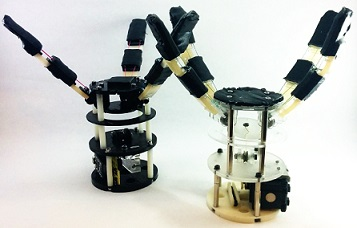
\includegraphics[width=10cm]{figures/Intro/RobotHands.jpg}
 	\end{center}
	\caption{Two different versions of the proposed robot hands are depicted.}
	\label{RobotHands}
\end{figure}

To name a few, some of the possible applications are: 1) for autonomous grasping and teleoperation/telemanipulation studies, 2) as end-effectors of humanoid robots, 3) for mobile and aerial vehicle platforms that can be modified to be grasping capable, 4) for educational purposes, as they provide a low-cost solution for highly intriguing robotics lessons, 5) or even as affordable myoelectric prostheses that will assist amputees in everyday life tasks, helping them regain part of their lost dexterity.  The presented robot hands have been developed through the \href{www.openbionics.org}{OpenBionics (www.openbionics.org)} initiative \cite{Liarokapis2014ASURRW}, which was inspired by the \href{http://www.eng.yale.edu/grablab/openhand/}{Yale Open Hand Project} \cite{Ma2013ICRA}.

\newpage

\section{Design}

\subsection{Robot Finger Structure}

 In this section we present the robot finger structure and we explain the design choices made. The proposed design is based on the following simple/bioinspired idea: to structurally reproduce the flexion/extension motions of human fingers, using steady elastomer materials (that introduce also compliance) for a passive extension and cables driven through low-friction tubes for the flexion. These design choices produce a simple mechanism capable to reproduce the agonist/antagonist behavior of human hand, exerting at the same time adequate forces. More details regarding the theoretical foundations and the design choices made can be found in \cite{Zisimatos2014IROS}.\\

\begin{wrapfigure}{r}{0.5\textwidth}
 	\vspace{10pt}
 	\begin{center}
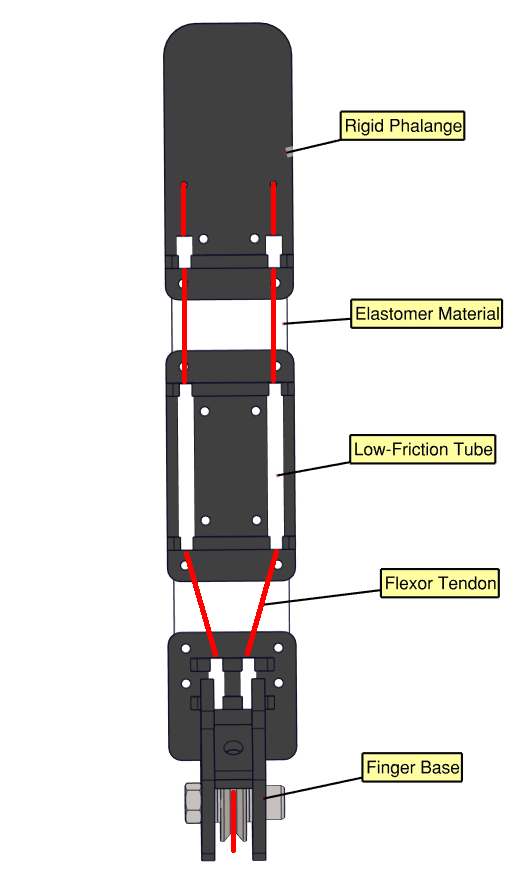
\includegraphics[width=7cm]{figures/Intro/Fig1-2.png}
 	\end{center}
 	\vspace{0pt}
 	\caption{The structure of the robot finger.}
	\label{Finger}
 	\vspace{0pt}
\end{wrapfigure}

For the elastomer material, we use appropriate silicone sheets which add adaptability to the structure and provide a more robust and stable behavior even when attempting to grasp objects of complex shapes \cite{DollarTM2006}. \\
The stiffness of the finger joints can be modeled as a stiffness matrix with non-zero values in its diagonal, which allows the robot finger to adapt to objects of different shapes. On the other hand, in manipulation tasks, the uncontrolled out-of-plane motion of the fingers, is typically undesired. In order to balance the two requirements we used a similar tendon routing with Awiwi Hand  \cite{GrebensteinThesis}, splitting from one tendon to two as you can see in Fig. \ref{Finger}. \\
Deformable material is attached at the fingertips. The deformations that arise during contact with the grasped object lead to larger contact areas, resulting in smoother contact force distributions and increased grasp stability, as discussed in \cite{deformableciocarlie2005}.
The rigid phalanges and some parts of the finger base were constructed with Plexiglas cut with a laser cutting machine. It should be noted though, that the hereby proposed design can be implemented with any kind of plastic and of course with the desired dimensions. For the assembly of the robot fingers we use fishing line and needles in order to stitch the silicone sheets onto the rigid links (the links have appropriate holes by design).\\
In order to minimize the friction in the tendon transmission system we use low-friction tubes and a pulley mounted inside the finger base. Therefore the Dyneema fishing line, used as flexor tendon, moves freely within the tendon routing system.\\


\newpage

\subsection{A Robot Hand Basis that Provides Modularity}

The proposed basis is equipped with 5 slots and can be used for attaching a total of four fingers, as depicted in Fig. \ref{Modular Base}. 
More specifically, robot hands with various geometries of finger base frames can be developed. Those hands are capable of grasping various everyday life objects and each one is specialized for executing different types of grasping tasks. This reflects the basic idea for the presented design, that someone can create multiple, low-cost, task-specific robot hands, instead of one that is complex and expensive.\\

\begin{figure*}[h!]
\begin{center}
\begin{tabular}{  c  c  }
{\bf{Two Fingers}} & {\bf{Three Fingers}} \\ 
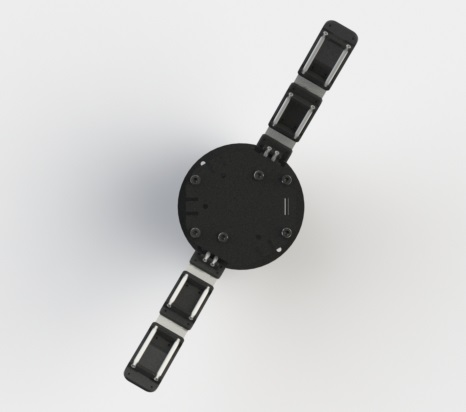
\includegraphics[height=3cm,width=3cm]{figures/Intro/Fig1-3-1.jpg}&
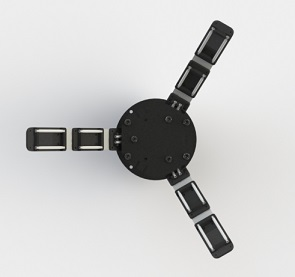
\includegraphics[height=3cm,width=3cm]{figures/Intro/Fig1-3-2.jpg} \\ 
{\bf{Four Fingers v1}} & {\bf{Four Fingers v2}}\\ 
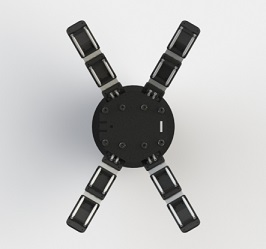
\includegraphics[height=3cm,width=3cm]{figures/Intro/Fig1-3-3.jpg}&
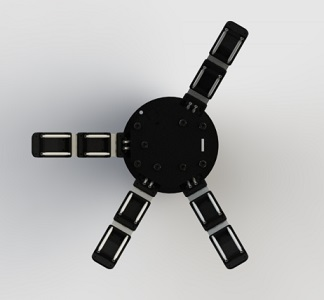
\includegraphics[height=3cm,width=3cm]{figures/Intro/Fig1-3-4.jpg}\\ 
\end{tabular}
\end{center}
\caption{Different robot hands created using identical modular fingers and the robot hand basis. One two-fingered, one three-fingered and two versions of four-fingered robot hands are depicted.} 
\label{Modular Base}
\end{figure*}

\subsection{A Disk Shaped Differential Mechanism}

\begin{wrapfigure}{l}{0.5\textwidth}
 	\vspace{0pt}
 	\begin{center}
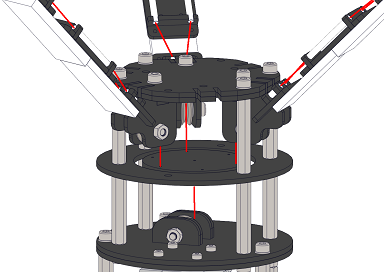
\includegraphics[width=6cm]{figures/Intro/Fig1-4.png}
 	\end{center}
 	\vspace{0pt}
 	\caption{The disk-shaped differential mechanism used in our robot hands.}
	\label{Disk}
 	\vspace{0pt}
\end{wrapfigure}

A disk-shaped differential mechanism has been developed to connect all the independent finger cables with the actuator (servo motor). The differential mechanism allows for independent finger flexions in case that one or multiple fingers have stopped moving, due to workspace constraints or in case that they are already in contact with the object surface. The mechanism is simple since it consists of a few simple parts (a Plexiglas disk, the dyneema fishing line and pulleys) and requires relatively small space in order to perform efficiently. Also, the differential disk moves in the air without being guided by sliders in an effort to minimize friction in the tendon routing system. Our differential mechanism is a variant of the whiffle tree (or seesaw) mechanism \cite{BirglenIJRR2006}.

\newpage

\section{Robot Hand Specifications}

In this section we present the robot hand specifications, i.e., the physical characteristics (Table \ref{Specs}, finger workspace and forces), design parameters 
(Table \ref{Parameters}) and grasping capabilities. All features refer to a 4-fingered robot hand with the Dynamixel AX12A actuator. All other designs presented, have lower weight but similar characteristics. \\

\subsection{Robot Hand Physical Characteristics}

In Table \ref{Specs}, the basic characteristics (dimensions and weight) of a four fingered robot hand version (V1) shown in Fig. \ref{Modular Base}, are presented.

\begin{table}[h!]
\caption{Robot Hand Physical Characteristics} 
\label{Specs}
\begin{center}
	\begin{tabular}{ | l | l | }
	\hline
 	\multicolumn{2}{|c|}{\bf{Four Fingered Robot Hand V1}} \\
	\hline
	Actuators & 1 \\ \hline
	Base Height (mm) & 110 \\ \hline
	Base Width (mm) & 77 \\ \hline
	Weight (g) & 280\\ \hline
    	\end{tabular}
\end{center}
\end{table}

\subsection{Design Parameters}

Our design is parametrized in the same way, reported in \cite{Ma2013ICRA}. The parameters are listed in Table \ref{Parameters}, to help the creator achieve optimized designs. More details can be found in \cite{DollarAR2005}. 

\begin{table}[h!]
\setlength{\belowcaptionskip}{-4pt}
\setlength{\abovecaptionskip}{-4pt}
\caption{Robot Hand Design Parameters} 
\label{Parameters}
\begin{center}
	\begin{tabular}{ | c | c | }
	\hline
	{\bf{Parameter}} & {\bf{Default Value}} \\ \hline
	KP, KD (flexure stiffness) (mm) &  3, 4 \\ \hline
	Stiffness Ratio & 2.37 \\ \hline
	KP Length, KD Length (mm) & 8, 8 \\ \hline
	RP, RD (transmission radii) (mm) & 2.25, 2.25 \\ \hline
	Transmission Ratio & 1 \\ \hline
	Finger Length (LP+LD) (mm) &  87.3 \\ \hline
	LP, LD (mm) & 44.1, 43.2 \\ \hline
	Linkage Ratio & 0.97 \\ \hline
	TP, TD (degrees) & 14 , 8 \\ \hline
	LB (mm) &  67\\ \hline
	Height (mm) &  12 \\ \hline
	Depth (mm) &  20 \\ \hline
	Pad Thickness (mm) & 6\\ \hline
    	\end{tabular}
\end{center}
\end{table}

Moreover, it should be noted that although in this project we are not proposing anthropomorphic robot hands, we used the metric presented in \cite{Liarokapis2013ICRA} in order to define the lengths for all phalanges and the relative positions of the finger base frames, maximizing humanlikeness of specific aspects of our design. Such a choice was made based on the hypothesis, that even if we design our simple robot hands as anthropomorphically as possible, we will maximize their ability to grasp objects created for the human hand. For our design we have used identical robot fingers following the dimensions of human index finger and for the distance between the opposing finger base frames we have selected the distance between the CMC of the thumb and the MCP of the index. This distance can be obtained using hand anthropometry studies \cite{BuchholzErgonomics1992}. More details can be found in \cite{Zisimatos2014IROS}. A recent study regarding prosthetic fingers can be found in \cite{Liarokapis2014EMBC}. 

\vspace{1cm}

\subsection{Finger Workspace}

The fingers' workspace is presented in Fig \ref{workspace}. The ratio graph between the first and the second angle is depicted in Fig. \ref{ratio}. The joint angles were captured experimentally, using markers at the joints and a vision system.

\begin{figure*}[h!]
\begin{center}
	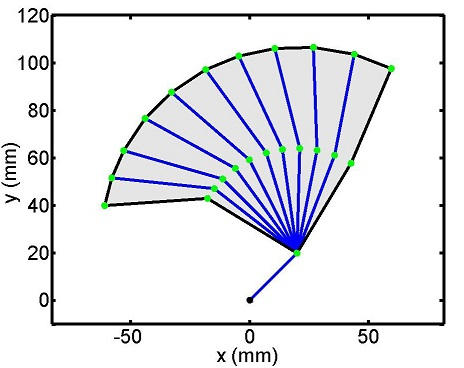
\includegraphics[width=8cm]{figures/Intro/Fig1-5-1.jpg}
\end{center}
\caption{ The finger workspace.} 
\label{workspace}
\end{figure*}

\begin{figure*}[h!]
\begin{center}
	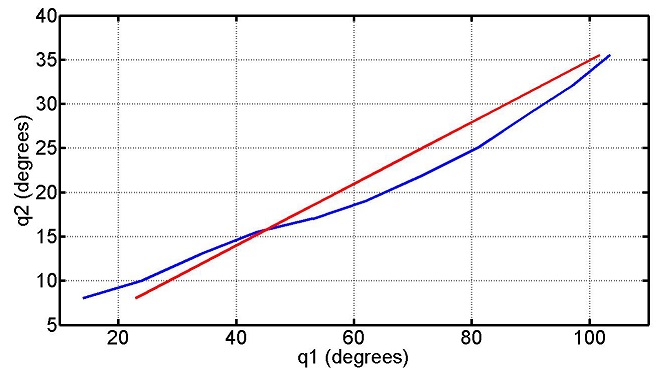
\includegraphics[width=10cm]{figures/Intro/Fig1-5-2.jpg}
\end{center}
\caption{The evolution of the ratio between the two angles. The ratio approximates a constant value of 2.86 (red line).} 
\label{ratio}
\end{figure*}

As we can see in Fig. \ref{workspace}, the proximal phalanx closes faster than the distal phalanx. This was achieved by selecting specific values of stiffness (KP, KD) for the two flexure joints (see Table \ref{Parameters} for details). Such a choice leads to more robust power grasps, as discussed in \cite{DollarTM2006}.

\vspace{1cm}

\subsection{Force Exertion Capability of Robot Fingers}
In order to evaluate the force exertion capability of the robot fingers, we measured the maximum force applied by the robot fingertips (distal phalanx) in two different configurations, as depicted in Fig. \ref{force1} and Fig. \ref{force2}. For each configuration, multiple experiments where conducted. The red lines represent the mean values and the blue dotted lines the min and max values per configuration. The high force values correspond to the 30\% flexed case and reach 18N (peak), with a standard low-cost servo. More details can be found in \cite{Zisimatos2014IROS}.

\begin{figure*}[h!]
\begin{center}
\begin{tabular}{  c  }
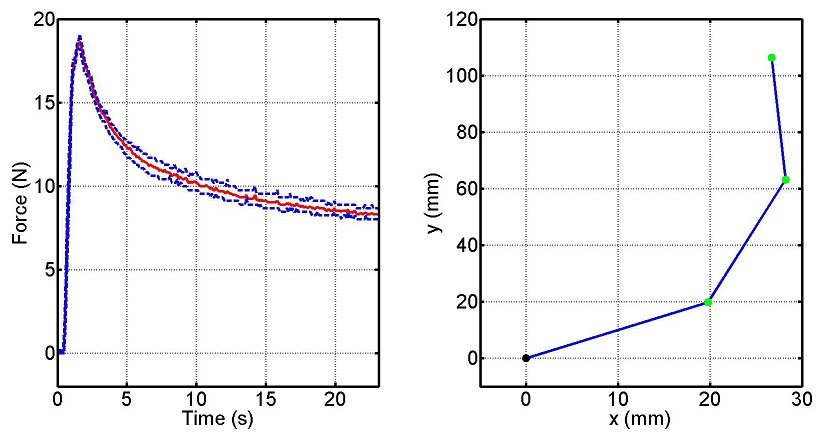
\includegraphics[width=12cm]{figures/Intro/Fig1-7.jpg}
\end{tabular}
\end{center}
\caption{Force exertion for the 30\% flexed configuration.}
\label{force1}
\end{figure*}

\begin{figure*}[h!]
\begin{center}
\begin{tabular}{  c  }
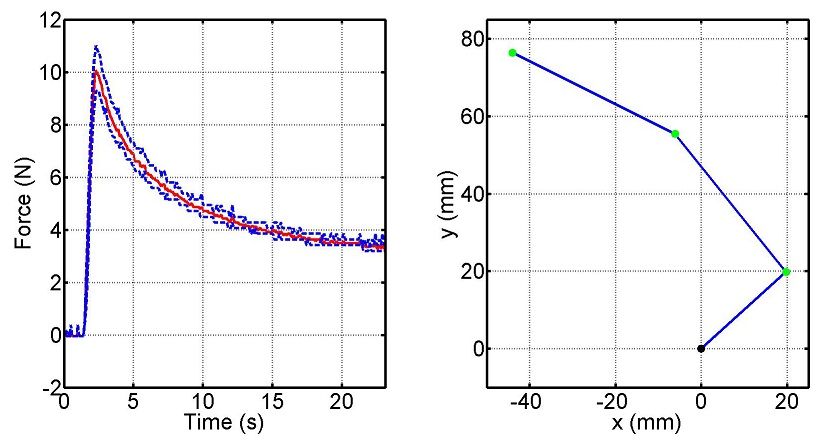
\includegraphics[width=12cm]{figures/Intro/Fig1-6.jpg}
\end{tabular}
\end{center}
\caption{Force exertion for the 70\% flexed configuration.} 
\label{force2}
\end{figure*}

As you can see  in Fig. \ref{force1} and Fig. \ref{force2} the forces drop at the 45\% of the maximum force applied and then they remain constant. This phenomenon is caused by the viscoelastic behavior of the silicone sheets \cite{DollarThesis}. \\

\newpage

\subsection{Experimental Validation of Robot Hands Efficiency}
\begin{figure*}[ht!]
\begin{center}
\begin{tabular}{ c }
\begin{tabular}{ c  c  c  c  c }
	\bf{Aerial Gripper} & \bf{Two Fingered} & \bf{Three Fingered}\\
	{Two Phalanges} & {Two Phalanges} & {Two Phalanges}\\

	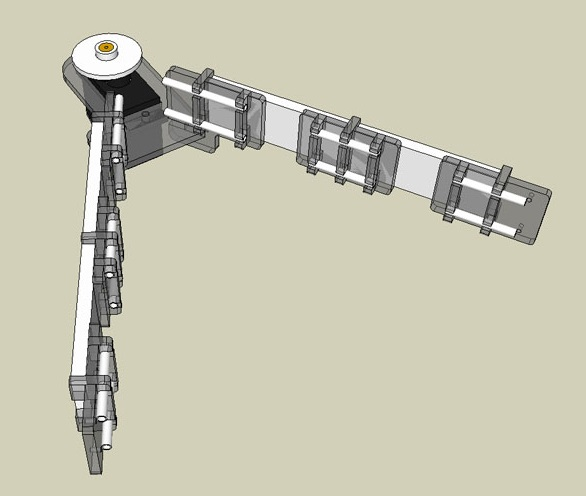
\includegraphics[height=2.5cm,width=3cm]{figures/Intro/Aerial_Gripper.jpg}&
	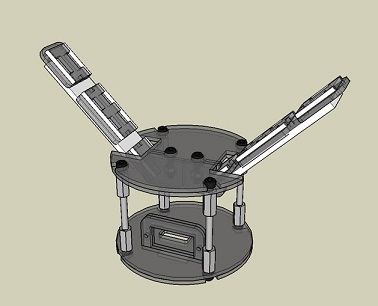
\includegraphics[height=2.5cm,width=3cm]{figures/Intro/RobotHand_2Fingered.jpg}&
	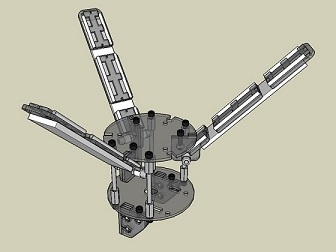
\includegraphics[height=2.5cm,width=3cm]{figures/Intro/RobotHand_3Fingered2Phalanges.jpg}\\

	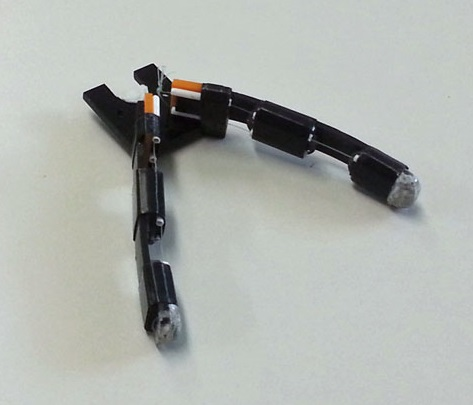
\includegraphics[height=2.5cm,width=3cm]{figures/Intro/Real_Aerial_Gripper.jpg}&
	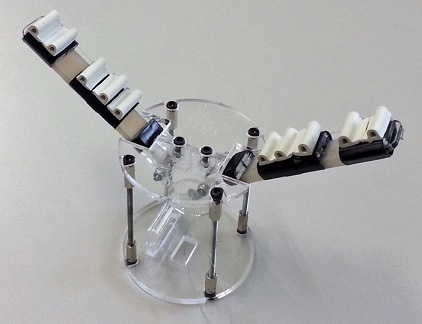
\includegraphics[height=2.5cm,width=3cm]{figures/Intro/RealRobotHand_2Fingered.jpg}&
	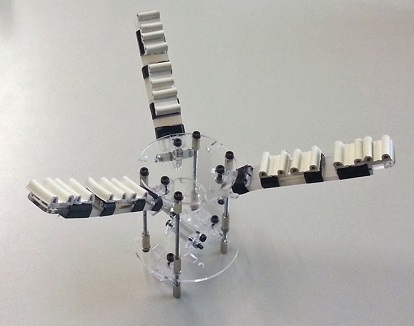
\includegraphics[height=2.5cm,width=3cm]{figures/Intro/RealRobotHand_3Fingered2Phalanges.jpg}\\
\end{tabular}\\
\begin{tabular}{ c  c  c  c  c }
	\bf{Three Fingered} & \bf{Four Fingered} \\
	{Three Phalanges} & {Two Phalanges} \\

	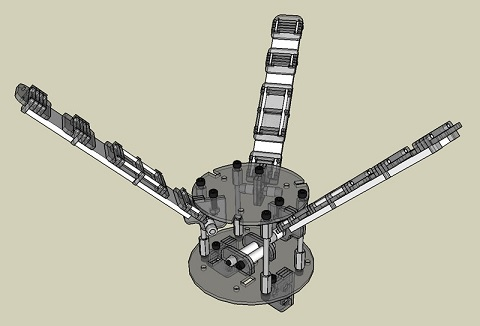
\includegraphics[height=2.5cm,width=3cm]{figures/Intro/RobotHand_3Fingered3Phalanges.jpg}&
	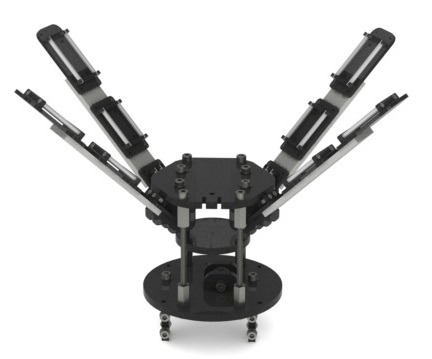
\includegraphics[height=2.5cm,width=3cm]{figures/Intro/RobotHand.jpg}\\

	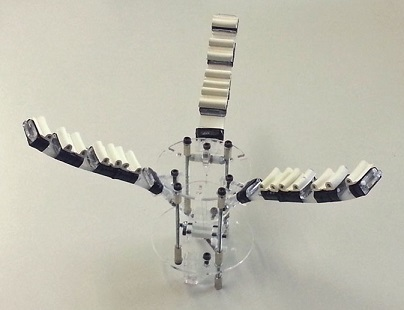
\includegraphics[height=2.5cm,width=3cm]{figures/Intro/RealRobotHand_3Fingered3Phalanges.jpg}&
	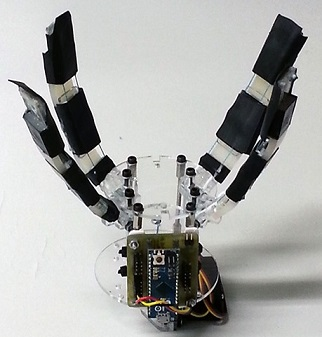
\includegraphics[height=2.5cm,width=2.5cm]{figures/Intro/RealRobotHand_4Fingered2Phalanges.jpg}\\
\end{tabular} \\
\end{tabular}
\end{center}
\caption{Different robot hand models and robot hands created with the design directions provided, are depicted. } 
\label{RobotHands}
\end{figure*}

In order to experimentally validate the efficiency of the aforementioned design, we have developed different types of robot hands depicted in Fig. \ref{RobotHands} and we have conducted various experiments, with different applications in mind. The videos of the conducted experiments, can be found at the following URLs:

\begin{center}
Different applications:
{\url{https://www.youtube.com/watch?v=yEANsfaE1gs}}\\
Autonomous grasp planning:
{\url{https://www.youtube.com/watch?v=xs2CC9QLuFc}}\\
Grebenstein test:
{\url{https://www.youtube.com/watch?v=bniHWeXpX0A}}\\
\end{center}

More details about the experiments and the possible applications, can be found in \cite{Zisimatos2014IROS}, as well as at the official website of the OpenBionics initiative:

\begin{center}
{\url{http://www.openbionics.org}}
\end{center} 

\newpage
